\documentclass{standalone}
\usepackage{tikz}
\usetikzlibrary{patterns, positioning}
\usepackage[sfdefault]{ClearSans} %% option 'sfdefault' activates Clear Sans as the default text font
\usepackage[T1]{fontenc}

\begin{document}
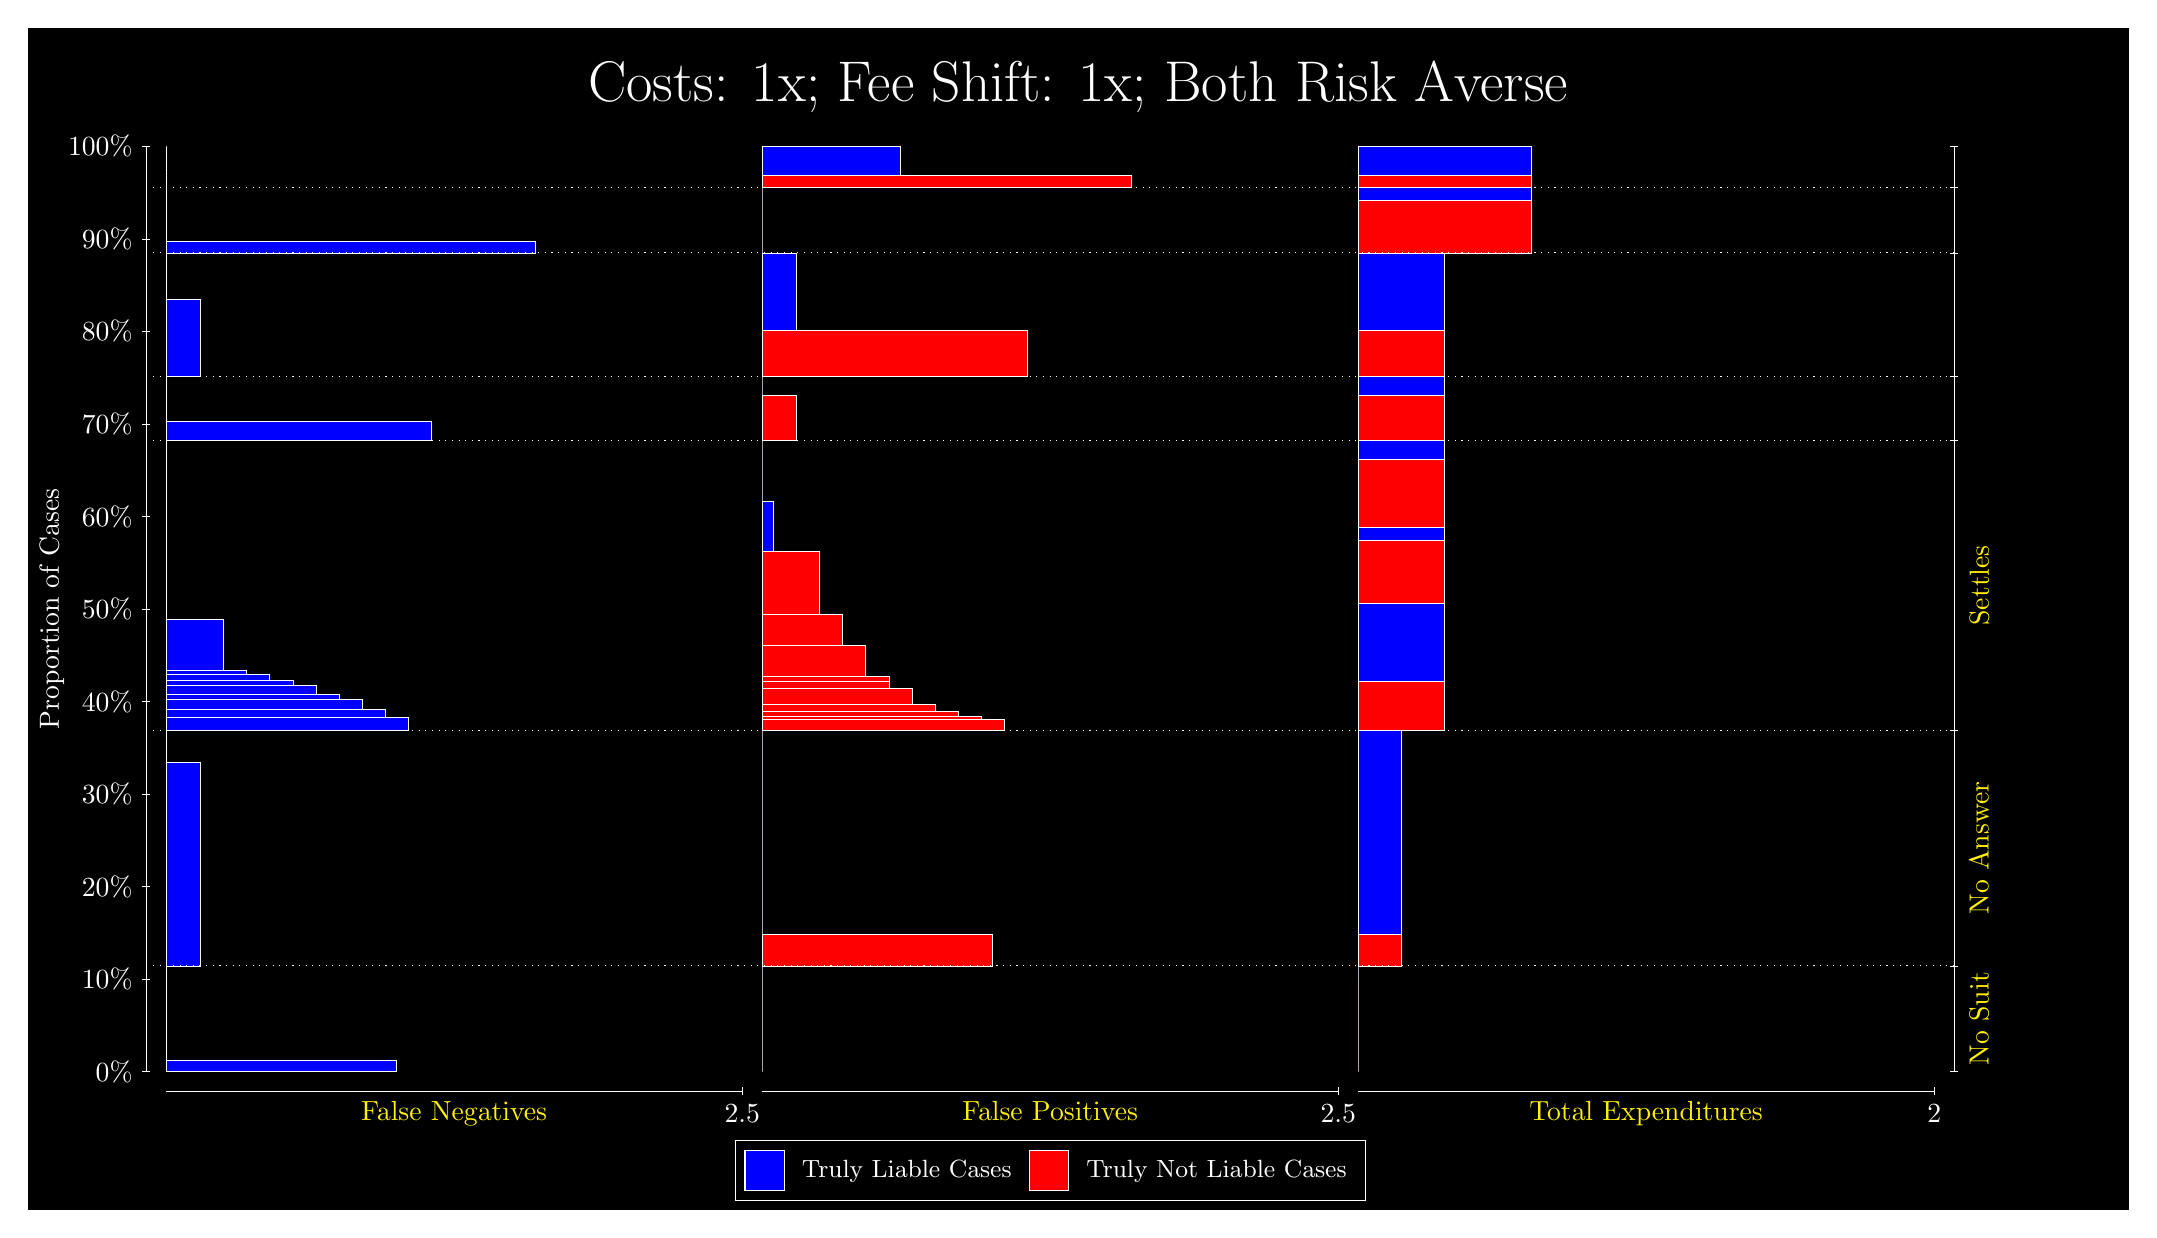
\begin{tikzpicture}
\draw[fill=black] (0,0) rectangle (26.667,15);
\draw[text=white] (0,13.5) rectangle (26.667,15) node[midway] {\huge Costs: 1x; Fee Shift: 1x; Both Risk Averse};
\draw[white, very thin] (1.5,1.75) -- (1.5,13.5);
\node[rotate=90, text=white, anchor=center] at (0.3, 7.625) {Proportion of Cases};
\draw[white, very thin] (1.45,1.75) -- (1.55,1.75);
\node[text=white, anchor=east] at (1.45, 1.75) {0\%};
\draw[white, very thin] (1.45,2.925) -- (1.55,2.925);
\node[text=white, anchor=east] at (1.45, 2.925) {10\%};
\draw[white, very thin] (1.45,4.1) -- (1.55,4.1);
\node[text=white, anchor=east] at (1.45, 4.1) {20\%};
\draw[white, very thin] (1.45,5.275) -- (1.55,5.275);
\node[text=white, anchor=east] at (1.45, 5.275) {30\%};
\draw[white, very thin] (1.45,6.45) -- (1.55,6.45);
\node[text=white, anchor=east] at (1.45, 6.45) {40\%};
\draw[white, very thin] (1.45,7.625) -- (1.55,7.625);
\node[text=white, anchor=east] at (1.45, 7.625) {50\%};
\draw[white, very thin] (1.45,8.8) -- (1.55,8.8);
\node[text=white, anchor=east] at (1.45, 8.8) {60\%};
\draw[white, very thin] (1.45,9.975) -- (1.55,9.975);
\node[text=white, anchor=east] at (1.45, 9.975) {70\%};
\draw[white, very thin] (1.45,11.15) -- (1.55,11.15);
\node[text=white, anchor=east] at (1.45, 11.15) {80\%};
\draw[white, very thin] (1.45,12.325) -- (1.55,12.325);
\node[text=white, anchor=east] at (1.45, 12.325) {90\%};
\draw[white, very thin] (1.45,13.5) -- (1.55,13.5);
\node[text=white, anchor=east] at (1.45, 13.5) {100\%};

\draw[white, very thin] (24.457,1.75) -- (24.457,13.5);
\draw[white, very thin] (24.407,1.75) -- (24.507,1.75);
\node[anchor=west] at (24.407, 1.75) {};
\draw[white, very thin] (24.407,3.0925) -- (24.507,3.0925);
\node[anchor=west] at (24.407, 3.0925) {};
\draw[white, very thin] (24.407,6.0832) -- (24.507,6.0832);
\node[anchor=west] at (24.407, 6.0832) {};
\draw[white, very thin] (24.407,9.7653) -- (24.507,9.7653);
\node[anchor=west] at (24.407, 9.7653) {};
\draw[white, very thin] (24.407,10.577) -- (24.507,10.577);
\node[anchor=west] at (24.407, 10.577) {};
\draw[white, very thin] (24.407,12.146) -- (24.507,12.146);
\node[anchor=west] at (24.407, 12.146) {};
\draw[white, very thin] (24.407,12.974) -- (24.507,12.974);
\node[anchor=west] at (24.407, 12.974) {};
\draw[white, very thin] (24.407,13.5) -- (24.507,13.5);
\node[anchor=west] at (24.407, 13.5) {};

\draw[white, very thin, fill=blue] (1.75,1.75) rectangle (4.6775,1.8912);
\draw[white, very thin, fill=red] (1.75,1.8912) rectangle (1.75,3.0925);
\draw[white, very thin, fill=blue] (1.75,3.0925) rectangle (2.1891,5.6782);
\draw[white, very thin, fill=red] (1.75,5.6782) rectangle (1.75,6.0832);
\draw[white, very thin, fill=blue] (1.75,6.0832) rectangle (4.8239,6.251);
\draw[white, very thin, fill=blue] (1.75,6.251) rectangle (4.5312,6.3515);
\draw[white, very thin, fill=blue] (1.75,6.3515) rectangle (4.2384,6.4753);
\draw[white, very thin, fill=blue] (1.75,6.4753) rectangle (3.9457,6.5356);
\draw[white, very thin, fill=blue] (1.75,6.5356) rectangle (3.6529,6.6578);
\draw[white, very thin, fill=blue] (1.75,6.6578) rectangle (3.3602,6.721);
\draw[white, very thin, fill=blue] (1.75,6.721) rectangle (3.0674,6.7934);
\draw[white, very thin, fill=blue] (1.75,6.7934) rectangle (2.7746,6.8507);
\draw[white, very thin, fill=blue] (1.75,6.8507) rectangle (2.4819,7.4889);
\draw[white, very thin, fill=red] (1.75,7.4889) rectangle (1.75,9.7653);
\draw[white, very thin, fill=blue] (1.75,9.7653) rectangle (5.1167,10.004);
\draw[white, very thin, fill=red] (1.75,10.004) rectangle (1.75,10.577);
\draw[white, very thin, fill=blue] (1.75,10.577) rectangle (2.1891,11.552);
\draw[white, very thin, fill=red] (1.75,11.552) rectangle (1.75,12.146);
\draw[white, very thin, fill=blue] (1.75,12.146) rectangle (6.4341,12.3);
\draw[white, very thin, fill=red] (1.75,12.3) rectangle (1.75,12.974);
\draw[white, very thin, fill=red] (1.75,12.974) rectangle (1.75,13.127);
\draw[white, very thin, fill=blue] (1.75,13.127) rectangle (1.75,13.5);
\draw[white, very thin, fill=red] (9.3189,1.75) rectangle (9.3189,2.9512);
\draw[white, very thin, fill=blue] (9.3189,2.9512) rectangle (9.3189,3.0925);
\draw[white, very thin, fill=red] (9.3189,3.0925) rectangle (12.246,3.4975);
\draw[white, very thin, fill=blue] (9.3189,3.4975) rectangle (9.3189,6.0832);
\draw[white, very thin, fill=red] (9.3189,6.0832) rectangle (12.393,6.2229);
\draw[white, very thin, fill=red] (9.3189,6.2229) rectangle (12.1,6.2656);
\draw[white, very thin, fill=red] (9.3189,6.2656) rectangle (11.807,6.3283);
\draw[white, very thin, fill=red] (9.3189,6.3283) rectangle (11.515,6.4188);
\draw[white, very thin, fill=red] (9.3189,6.4188) rectangle (11.222,6.616);
\draw[white, very thin, fill=red] (9.3189,6.616) rectangle (10.929,6.7019);
\draw[white, very thin, fill=red] (9.3189,6.7019) rectangle (10.929,6.7641);
\draw[white, very thin, fill=red] (9.3189,6.7641) rectangle (10.636,7.1579);
\draw[white, very thin, fill=red] (9.3189,7.1579) rectangle (10.344,7.5557);
\draw[white, very thin, fill=red] (9.3189,7.5557) rectangle (10.051,8.3596);
\draw[white, very thin, fill=blue] (9.3189,8.3596) rectangle (9.4652,8.9978);
\draw[white, very thin, fill=blue] (9.3189,8.9978) rectangle (9.3189,9.7653);
\draw[white, very thin, fill=red] (9.3189,9.7653) rectangle (9.758,10.338);
\draw[white, very thin, fill=blue] (9.3189,10.338) rectangle (9.3189,10.577);
\draw[white, very thin, fill=red] (9.3189,10.577) rectangle (12.686,11.17);
\draw[white, very thin, fill=blue] (9.3189,11.17) rectangle (9.758,12.146);
\draw[white, very thin, fill=red] (9.3189,12.146) rectangle (9.3189,12.819);
\draw[white, very thin, fill=blue] (9.3189,12.819) rectangle (9.3189,12.974);
\draw[white, very thin, fill=red] (9.3189,12.974) rectangle (14.003,13.127);
\draw[white, very thin, fill=blue] (9.3189,13.127) rectangle (11.075,13.5);
\draw[white, very thin, fill=red] (16.888,1.75) rectangle (16.888,2.9512);
\draw[white, very thin, fill=blue] (16.888,2.9512) rectangle (16.888,3.0925);
\draw[white, very thin, fill=red] (16.888,3.0925) rectangle (17.437,3.4975);
\draw[white, very thin, fill=blue] (16.888,3.4975) rectangle (17.437,6.0832);
\draw[white, very thin, fill=red] (16.888,6.0832) rectangle (17.986,6.7019);
\draw[white, very thin, fill=blue] (16.888,6.7019) rectangle (17.986,7.6939);
\draw[white, very thin, fill=red] (16.888,7.6939) rectangle (17.986,8.4977);
\draw[white, very thin, fill=blue] (16.888,8.4977) rectangle (17.986,8.6655);
\draw[white, very thin, fill=red] (16.888,8.6655) rectangle (17.986,9.5193);
\draw[white, very thin, fill=blue] (16.888,9.5193) rectangle (17.986,9.7653);
\draw[white, very thin, fill=red] (16.888,9.7653) rectangle (17.986,10.338);
\draw[white, very thin, fill=blue] (16.888,10.338) rectangle (17.986,10.577);
\draw[white, very thin, fill=red] (16.888,10.577) rectangle (17.986,11.17);
\draw[white, very thin, fill=blue] (16.888,11.17) rectangle (17.986,12.146);
\draw[white, very thin, fill=red] (16.888,12.146) rectangle (19.083,12.819);
\draw[white, very thin, fill=blue] (16.888,12.819) rectangle (19.083,12.974);
\draw[white, very thin, fill=red] (16.888,12.974) rectangle (19.083,13.127);
\draw[white, very thin, fill=blue] (16.888,13.127) rectangle (19.083,13.5);
\draw[white, dotted] (1.5,3.0925) -- (24.457,3.0925);
\draw[white, dotted] (1.5,6.0832) -- (24.457,6.0832);
\draw[white, dotted] (1.5,9.7653) -- (24.457,9.7653);
\draw[white, dotted] (1.5,10.577) -- (24.457,10.577);
\draw[white, dotted] (1.5,12.146) -- (24.457,12.146);
\draw[white, dotted] (1.5,12.974) -- (24.457,12.974);
\draw[white, very thin] (1.75,1.5) -- (9.0689,1.5);
\node[text=yellow, anchor=north] at (5.4094, 1.5) {False Negatives};
\draw[white, very thin] (9.0689,1.45) -- (9.0689,1.55);
\node[text=white, anchor=north] at (9.0689, 1.45) {2.5};

\draw[white, very thin] (9.3189,1.5) -- (16.638,1.5);
\node[text=yellow, anchor=north] at (12.978, 1.5) {False Positives};
\draw[white, very thin] (16.638,1.45) -- (16.638,1.55);
\node[text=white, anchor=north] at (16.638, 1.45) {2.5};

\draw[white, very thin] (16.888,1.5) -- (24.207,1.5);
\node[text=yellow, anchor=north] at (20.547, 1.5) {Total Expenditures};
\draw[white, very thin] (24.207,1.45) -- (24.207,1.55);
\node[text=white, anchor=north] at (24.207, 1.45) {2};

\node[text=yellow, centered, rotate=90] at (24.777, 2.4212) {No Suit};
\node[text=yellow, centered, rotate=90] at (24.777, 4.5878) {No Answer};
\node[text=yellow, centered, rotate=90] at (24.777, 7.9242) {Settles};





\draw (12.978300999999998,1.5) node[draw=none] (baseCoordinate) {};
\begin{scope}[align=center]
        \matrix[scale=0.5, draw=white, below=0.5cm of baseCoordinate, nodes={draw}, column sep=0.1cm]{
            \node[rectangle, draw, minimum width=0.5cm, minimum height=0.5cm, fill=blue] {}; &
            \node[draw=none, font=\small, text=white] (B) {Truly Liable Cases}; &
            \node[rectangle, draw, minimum width=0.5cm, minimum height=0.5cm, fill=red] {}; &
            \node[draw=none, font=\small, text=white] (B) {Truly Not Liable Cases}; \\
            };
\end{scope}

\end{tikzpicture}
\end{document}